En este capítulo se hablará sobre la implementación realizada. Primero, se introducirá el \emph{hardware} utilizado. Luego, se explicará de que manera se procesaron las distintas señales, desde la obtención de las mismas hasta las características y clasificadores utilizados. Finalmente, se hablará de los universos 3D interactivos desarrollados. Los universos 3D fueron desarrollados en el lenguaje \emph{C\#} en \emph{Unity}.

\section{Hardware}

Para la elección del \emph{hardware} se tuvieron en cuenta distintos criterios. Principalmente se busco un compromiso entre costo y fiabilidad pero también se tuvo en cuenta su facilidad de uso.

\subsection{EEG}

En el caso de EEG, se decidió utilizar el \emph{Muse Brainsensing Headband}. Este dispositivo cuenta cuenta con siete electrodos y diversas funcionalidades. En la figura \ref{fig:muse-electrodes} se puede observar la configuración del dispositivo. Cuenta con tres electrodos de referencia sobre la frente, dos electrodos frontales y dos electrodos en las orejas. Los electrodos de referencia se utilizan para medir el nivel de potencial eléctrico. Es decir, el potencial de los restantes electrodos, se mide en base a los electrodos de referencia.

\begin{figure}[H]
	\centering
    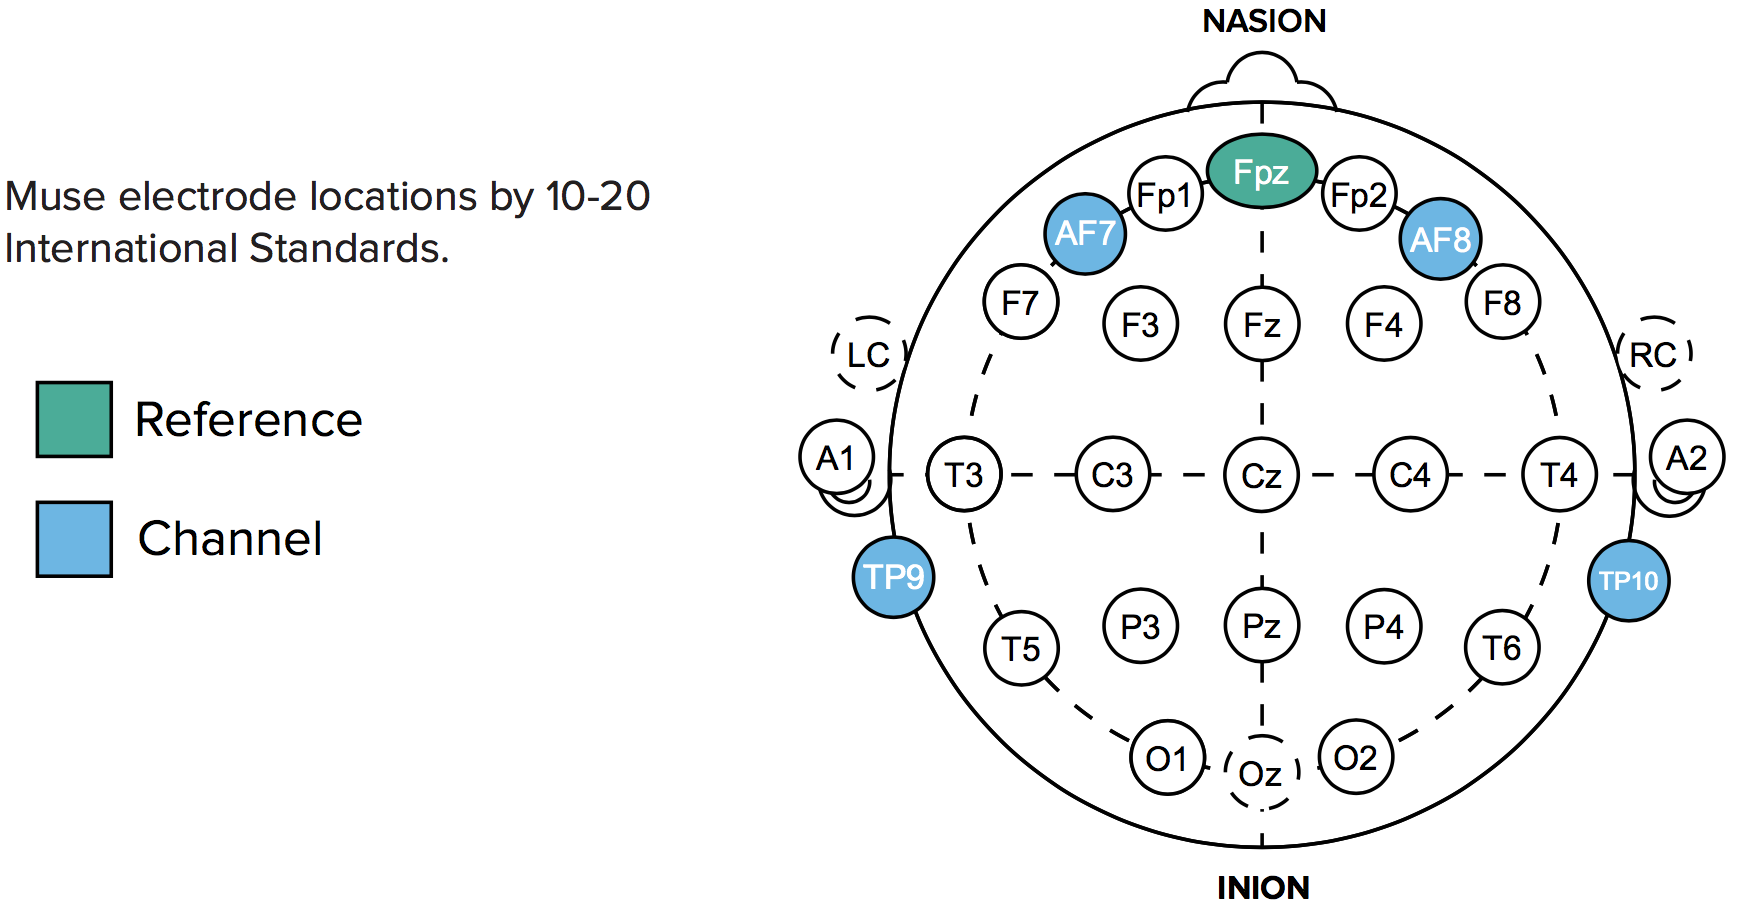
\includegraphics[width=0.8\textwidth]{muse-electrodes.png}
    \caption{Diagrama de la ubicación de los electrodos en el \emph{Muse Brainsensing Headband}. AF7 y AF8 son los electrodos frontales, TP9 y TP10 los electrodos en las orejas y Fpz representa los tres electrodos de referencia \cite{muse-hardware}.}
	\label{fig:muse-electrodes}
\end{figure}

El dispositivo tiene una frecuencia de muestreo de $ 256 \, Hz$. Además cuenta con acelerómetro y giroscopio lo que permite medir la orientación del usuario. También cuenta con un puerto micro USB y \emph{bluetooth}. Permite acceder a la información bruta de cada electrodo por lo que se obtienen cinco valores. Cuatro de de los electrodos frontales y de las orejas, y el restante se obtiene de los tres electrodos de referencia. También brinda algunas facilidades como realizar la Transformada de \emph{Fourier},  calcular la potencia de las bandas ($\alpha$, $\beta$, $\delta$, $\theta$ y $\gamma$), entre otros.

Para los desarrolladores, cuenta con \emph{SDK} para \emph{Windows} y \emph{Unity} y cuenta con aplicaciones multiplataforma para poder acceder a los datos. Una forma de acceder a los datos es a través de \emph{OSC} (\emph{Open Sound Control}. \emph{OSC} es un protocolo que corre sobre UDP y permite el \emph{stream} continuo de datos.

\subsection{EMG} \label{emg-hardware}

Para la lectura de señales EMG, se opto por utilizar la plataforma Arduino, con un modulo adicional diseñado para la captura de señales EMG y EKG.  Arduino es una plataforma que consiste en varios micro controladores de diseño abierto (\emph{Open Source Hardware}), y un software que permite programarlos de forma fácil y rápida utilizando el lenguaje de progamación \emph{C++}.

El modelo de Arduino elegido fue el \emph{Arduino Mega 2560}, que cuenta con un procesador que opera a $16\, MHz$, y cuenta con $256 Kb$ de memoria para programas, lo cual prácticamente permite trabajar sin restricciones de memoria en mente. A su vez, el modulo adicional elegido fue el \emph{Olimex SHIELD-EKG-EMG}, que trae electrodos superficiales que pueden ser ubicados sobre la piel del musculo que se intenta monitorear.  Los electrodos cuentan con tres terminales, marcadas con las letras $L$ (izquierda), $R$ (derecha) y $D$ (referencia) (figura \ref{fig:emg-electrodes}).

\begin{figure}[H]
	\centering
    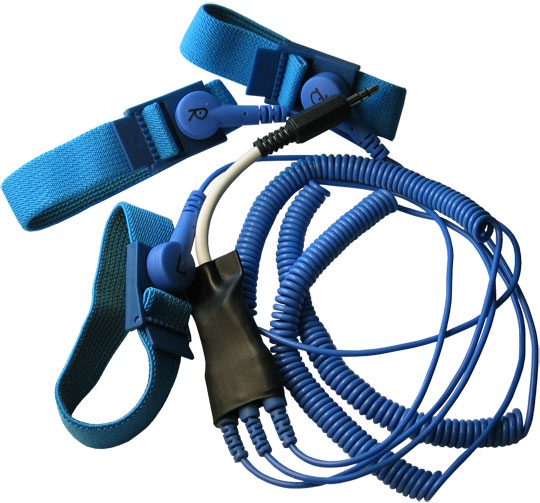
\includegraphics[width=0.5\textwidth]{electrodes.jpg}
    \caption{Electrodos superficiales para el modulo \emph{Olimex SHIELD-EKG-EMG}.}
	\label{fig:emg-electrodes}
\end{figure}

Para poder leer las señales EMG, se debe preparar el sistema de monitoreo.  Primero, se debe montar el modulo EMG sobre el micro controlador \emph{Arduino}.  Luego, las terminales $L$ y $R$ se deben posicionar sobre la piel del musculo a monitorear, y la terminal $D$ debe ser posicionada sobre una superficie del cuerpo a utilizar como referencia, que preferiblemente no contenga musculos, o tenga musculos no relacionados a los de las otras dos terminales (a este circuito se le llama \emph{Driven Right Leg Circuit} en inglés). En este proyecto, se opto por medir la actividad muscular de un brazo, junto a la mano, al formar un puño cerrado apretado. Por lo tanto, los electrodos fueron colocados sobre el músculo flexor común superficial de los dedos, que se encuentra sobre la cara anterior de antebrazo\cite{emg-signals-wrist}. Una vez realizados los pasos anteriores, se puede proceder a conectar el micro controlador a la computadora vía un cable USB 2.0.

\subsection{EKG}

TODO

\section{Obtención y Procesamiento de Señales}

Para cada uno de los sensores se evaluaron y aplicaron distintas alternativas sobre como procesar la señal.

\subsection{EEG}

Para leer la señal se decidió utilizó \emph{OSC}. Se tomo esta decisión ya que al momento de iniciar el proyecto, el \emph{SDK} para Windows se encontraba en estado beta por lo que no era confiable. Además implicaba un desarrollo en el lenguaje \emph{C} mientras que el desarrollo se encontraba en \emph{C\#} y, como solo se encontraba disponible para \emph{Windows}, no permitía que el proyecto sea multiplataforma. Tampoco se utilizó el \emph{SDK} para \emph{Unity}, ya que este era únicamente para dispositivos móviles.

Una gran desventaja de este dispositivo, es que no cuenta con soporte para la aplicación \emph{MuseIO}, que permite obtener paquetes \emph{OSC} a través de la computadora. Por este motivo, se terminó utilizando una aplicación móvil llamada \emph{Muse Monitor}, que nos permitió conectar el dispositivo al teléfono celular y desde allí enviar los paquetes \emph{OSC} hacia la computadora. En un principio se pensó que la latencia podría ser un problema ya que cada paquete debe realizar dos trayectos, primero desde el dispositivo hacia el teléfono celular y luego hacia la computadora, pero esto no fue un problema ya que el flujo de datos no era masivo y no eran de gran tamaño.

En un principio, se utilizó un \emph{framework} para procesar los paquetes \emph{OSC} pero este no resultó ser fiable. Se buscaron alternativas pero no hubo ninguna que cumpla con los estándares del equipo. Por este motivo, se desarrollo un procesador de paquetes \emph{OSC} propio. Esto implicó leer el estándar, comprender como funciona e implementarlo.
 
 Los estados que se buscaron detectar fueron ojos abiertos (A) y ojos cerrados (C). Por este motivo, la información que se necesitaba eran las ondas $\alpha$. Como se mencionó anteriormente, el dispositivo \emph{Muse} permitía acceder a la potencia de las ondas $\alpha$ con. Para obtener dichas ondas el dispositivo sigue el siguiente procedimiento:
 
 \begin{enumerate}
 \item Obtener una ventana $25$ muestras (pues envía $10$ muestras por segundo y el sensor obtiene $256$ muestras por segundo) y aplicar la función de ventana $Hann$.
 \item Obtener la Transformada de \emph{Fourier} de la ventana.
 \item Aplicar un filtro pasa banda para utilizar únicamente las frecuencias de interés ( $ 8 \, Hz \leq f \leq 13 \, Hz$).
 \item Realizar la DEP sobre esos valores. A diferencia de solo integrar, el dispositivo aplica $log_{10}$  a cada valor antes de realizar la integral.
 \end{enumerate}

El vector de características se confeccionó utilizando dos valores de \emph{Alpha} consecutivos, es decir, de la siguiente manera:

\[
  \vec{v}^{\, }=
  \left[ {\begin{array}{cc}
   \alpha_{i}  & \alpha_{i + 1}  \     \end{array} } \right]
\]

En la etapa de entrenamiento se le asignaba un estado a cada uno de estos vectores. La precisión obtenida con este método fue de entre un $65\%$ y un $70\%$. Esto se debe a que aún cuando el usuario se encontraba con los ojos abiertos, \emph{Alpha} alcanzaban valores tan altos como cuando el usuario se encontraba con los ojos cerrados debido a ruidos del sensor y a el hecho de que las bioseñales varían mucho. Se podía observar que el clasificador era muy preciso en detectar ojos cerrados pero muy impreciso en detectar ojos abiertos. La precisión en ojos cerrados era de un $99\%$ y en ojos abiertos de un $25\%$.

Para intentar mejorar la precisión, se decidió aumentar el tamaño de la ventana con la expectativa de que al tener una mayor cantidad de valores, los picos anómalos que se generaban cuando el usuario estaba con los ojos abiertos, se redujeran ya que, al contar con más muestras, además de obtener picos anómalos, se obtienen los valores que corresponden al estado de ojos abiertos. Se podría decir que los picos anómalos se promedian con más valores. Cuando se trabaja con bioseñales, cuantos más datos se tomen, más robusta será la clasificación. El problema es que para tomar más datos se necesita más tiempo. Entonces, aquí aparece un compromiso entre robustez y latencia. Como en este proyecto la utilización fue en tiempo real, hubo que considerar seriamente este compromiso. El dispositivo utiliza una frecuencia de $10 \, Hz$ para los valores de potencia de \emph{Alpha} y se necesitaba una frecuencia mayor, por lo que se decidió calcular dicha potencia utilizando los datos brutos. El dispositivo envía un arreglo de cinco elementos. Como se mencionó anteriormente, el quinto valor es de referencia por lo que se ignora en el procesamiento. El procedimiento implementado fue el siguiente:

 \begin{enumerate}
 \item Obtener una ventana $256$ muestras, es decir, un segundo.
 \item Obtener la Transformada de \emph{Fourier} de la ventana.
 \item Quedarse únicamente con las frecuencias $8 \, Hz-13 \, Hz$.
 \item Realizar la DEP sobre esos valores.
 \end{enumerate}
 
Este procedimiento se aplica por cada uno de los cuatro electrodos. Por lo que cada segundo, se cuenta con cuatro valores. El vector de características se forma con estos cuatro valores de la siguiente manera:
 
\[
  \vec{v}^{\, }=
  \left[ {\begin{array}{cccc}
   \alpha_{AF7}  & \alpha_{AF8} & \alpha_{TP9} & \alpha_{TP10}  \     \end{array} } \right]
\] 

Con este vector de características, se alcanzó una precisión de hasta un $ 85 \%$. Esto se debe a que, si bien empeoro la precisión de detectar ojos cerrados, incrementó notablemente la de ojos abiertos.
 
En la etapa de entrenamiento, en lugar de tomar todos los valores, se ignoran los valores de transición. Cuando se le indica al usuario que abra o cierre los ojos, se descartan dos segundos antes y después de la transición de estados. Esto se debe a que los valores que corresponden a la transición no son significativos. Los que realmente importan son cuando se está en un estado u otro.
 
\subsection{EMG}

Una vez preparado el sistema de monitoreo EMG descripto en la seccion \ref{emg-hardware}, se puede comenzar a leer los datos. Los micro controladores \emph{Arduino} permiten comunicarse a una computadora mediante un puerto de serie que es establecido a traves de la conexión USB.  Para poder leer del puerto de serie desde el sistema operativo, es necesario conocer los parametros de la conexión (velocidad, paridad, cantidad de bits de información, etc.), y el nombre del puerto de serie. Los valores utilizados fueron los predeterminados utilizados en el programa de ejemplo referenciado en el manual del módulo EMG\cite{olimex-manual}.

El dispositivo cuenta con una frecuencia de muestreo de $256\, Hz$. Por el teorema de muestreo de Nyquist-Shannon, esto quiere decir que dadas estas muestras, solo es posible reconstruir señales con frecuencias iguales o inferiores a $128\, Hz$. Teniendo esto en mente, el procedimiento llevado a cabo para leer los datos de EMG fueron los siguientes:

 \begin{enumerate}
 \item Obtener una ventana $128$ muestras, es decir, medio segundo.
 \item Obtener la Transformada de \emph{Fourier} de la ventana.
 \item Quedarse únicamente con las frecuencias en el rango de $50 \, Hz-128 \, Hz$. Las frecuencias en el rango de $128 \, Hz-150 \, Hz$ no son capturadas.
 \item Separar el rango de frecuencias resultante en dos mitades: $50 \, Hz-89 \, Hz$ y $90 \, Hz-128 \, Hz$.
 \item Realizar la DEP sobre ambas mitades por separado.
 \end{enumerate}

Luego de haber realizado los pasos mencionados, el resultado son dos valores numéricos representativos de la intensidad de la señal recibida.  Utilizando estos dos valores, se construyo el vector de características de la señal EMG. Con este vector, se lograron precisiones de predicción muy altas (superiores a $ 95 \%$), utilizando tiempos de entrenamiento de alrededor de $5$ minutos.

Para el entrenamiento, el procedimiento fue simple. Primero, se preparo el sistema de monitoreo EMG, y se colocaron los electrodos sobre la piel del los músculos mencionados en la sección \ref{emg-hardware}. Luego, con el brazo y mano relajados, se comenzó a entrenar un clasificador con las muestras leídas y procesadas. A continuación se procedió a tensar el brazo y cerrar la mano con fuerza, con tal de generar una diferencia de potencial significativa, en intervalos intermitentes de alrededor de $15$ segundos. Durante todo el proceso, se le informa al clasificador a que categoría pertenece cada dato ingresado (musculo tensionado o relajado).

Al igual que en EEG, al transicionar de un estado de tension de musculo a otro, se ignora cierta cantidad de muestras luego del momento de la transición, ya que solo son de interés los datos leídos al mantener un estado de tension constante. 

Al realizar los experimentos, se noto que ocasionalmente los datos leídos contenían grandes cantidades de ruido, por lo que eran prácticamente inutilizables. El problema encontrado fue que el sujeto conectado al modulo EMG no estaba eléctricamente aislado al suelo, lo cual introducía ruido a los valores leídos. El problema fue resuelto asegurándose de que el sujeto utilizara calzado con suficiente aislación eléctrica, como por ejemplo botas o zapatillas deportivas.

\subsection{EKG}

TODO

\section{Desarrollo de universos 3D interactivos}

TODO